\documentclass[12pt]{article}
\usepackage{amssymb,graphicx}
\usepackage{subfigure}
\usepackage[hyphens,obeyspaces,spaces]{url}
\usepackage{amsmath}
\usepackage{amsfonts}
\usepackage{amssymb}
\usepackage[T1]{fontenc}
\usepackage{carolmin}
\usepackage{t1enc}
\usepackage{color}
%\usepackagqe{times}
\usepackage{textcomp}
%\usepackage{natbib}
\usepackage[lined]{algorithm2e}

\def\eop{\hfill{$\vcenter{\hrule height1pt \hbox{\vrule width1pt
height5pt \kern5pt \vrule width1pt} \hrule height1pt}$}}

\newcommand{\bydef}{\mbox{$\:\stackrel{\triangle}{=}\:$}}
\newcommand{\insmat}[1]{\mathop{\rm {#1}}}  % for mathmode (with underlines)
\newcommand{\half}{{\textstyle\frac{1}{2}}}
\newcommand{\norm}[1]{\|#1\|}
\newcommand{\argmin}{\insmat{arg\,min}}
\newcommand{\argmax}{\insmat{arg\,max}}
\newcommand{\dist}{\insmat{dist\,}}
\newcommand{\aff}{\insmat{aff\,}}
\newcommand{\cl}{\insmat{cl\,}}
\newcommand{\conv}{\insmat{conv\,}}
\newcommand{\Qh}{\widehat{{\Omega}}}
\newcommand{\gammapQ}{\gamma_{p {\Omega}}}
\newcommand{\Pmu}{\mathbb{P}_\mu}
%\linespread{3.0} %For JOTA format


\begin{document}
%\noindent
%\begin{center}
%\large \textbf{Suboptimality of minmax MPC}
%\vspace{0.5cm}
%\noindent
%\vspace{0.5cm}
%\end{center}

\noindent
\begin{center}
 \textbf{MPC Path Planner}
\vspace{0.5cm}
\noindent
\vspace{0.5cm}
\end{center}
\textbf{This memo is only an idea sketch; it does not include detailed discussion.}
\\
\\ 
At current time, solve following optimization problem. $N$ is a horizon length, $m$ is the number of detected static and dynamic(moving) obstacles. For the simple notation, let initial time be $1$ for all time windows. The pair $z_k:=(x_k,y_k)$ is a position of vehicle at time $k$.$\tau^i_k$ is the position of the $i^{th}$ obstacle at time $k$. $T$ is a goal position that the ego vehicle wishes to arrive in the future. Fig.1 shows a concept of this approach.

\begin{figure}[h!]
\begin{centering}
	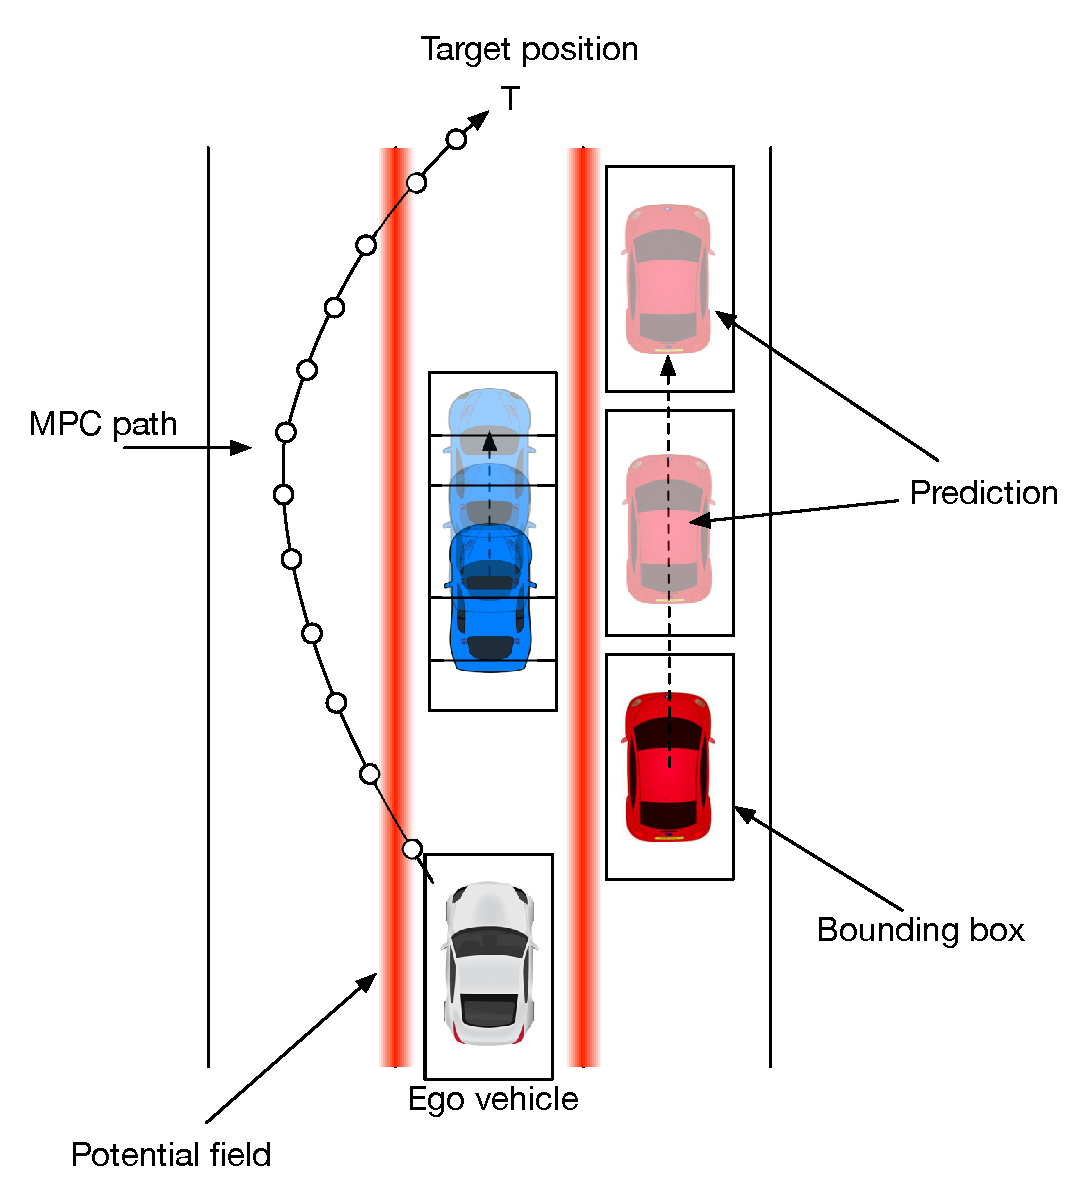
\includegraphics[width=11cm]{./Figures/mpc-path.eps}
\par\end{centering}
\caption{MPC path planning concept }
\end{figure}

\subsection*{Modeling}
Both ego vehicle and dynamic obstacles are unicycle model.
\begin{equation}
\begin{split}
&x_{k+1}=x_{k}+v_{k}\Delta \cos\theta_{k}(+\Delta^{2}\alpha_{k}\cos\theta_{k}),\\
&y_{k+1}=y_{k}+v_{k}\Delta \sin\theta_{k}(+\Delta^{2}\alpha_{k}\sin\theta_{k}),\\
&\theta_{k+1}=\theta_{k}+\Delta \omega_{k},\\
&v_{k+1}=v_{k}+\Delta \alpha_{k}\\
\end{split}
\end{equation}
Inputs are yaw rate $\omega$ and acceleration $\alpha$. High order terms () can be omitted for simplicity.
\subsection*{MPC formulation}
Inputs:
\begin{equation}
u=
\begin{Bmatrix}
\begin{bmatrix}
\alpha_1\\ 
\omega_1
\end{bmatrix}
\cdots
\begin{bmatrix}
\alpha_N\\ 
\omega_N
\end{bmatrix}
\end{Bmatrix}\in R^{2\times N}
\end{equation}
Optimization problem:
\begin{equation}
\begin{split}
&\min_{u\in U}\sum_{k=1}^Nw_{goal}D^2_k(z_k)+w_{acc}\|\ddot{z}_k \|^2+w_{jerk}\|\dddot{z_k} \|^2 + w_{yawr}\dot{\theta}^2+w_{lane}L(x_k,l_k,r_k)\\
s.t.&~~ \textit{Dynamics for ego and obstacle vehicles},\\
&~~ -\kappa_{max} \leq \kappa_k \leq k_{max},\\
&~~ -a_{max} \leq \|\ddot{z}_k \| \leq a_{max},\\
&~~ -\alpha_{max} \leq \|\dot{\theta}_k \| \leq \alpha_{max},\\
&~~ \|z_k-\tau^i_k \|_g\geq\epsilon,~~i\in \{1,2,\cdots, m \}
\end{split}
\end{equation}
where 
\begin{equation}
\kappa_k=\frac{\dot{x}_k\ddot{y}_k-\dot{y}_k\ddot{x}_k}{(\dot{x}_k^2+\dot{y}_k^2)^{\frac{1}{3}}}
\end{equation}
is a curvature of trajectory at time $k$.
\begin{equation}
D_k(z_k)=\|z_k - T \|
\end{equation}
is a distance to the goal position.

Penalties for left and right lane segments are as follow.
\begin{equation}
\label{penalty}
L(x_k,l_k,r_k) = \frac{\exp(-\alpha(\|x_k-l_k\|^2-s^2))}{1+\exp(-\alpha(\|x_k-l_k\|^2-s^2))} + \frac{\exp(-\alpha(\|x_k-r_k\|^2-s^2))}{1+\exp(-\alpha(\|x_k-r_k\|^2-s^2))},
\end{equation}
where
$l_k$ and $r_k$ are positions of left and the right lanes at time $k$, respectively. This could be defined as distances depending on FORD RNDF map data. $\|z_k-\tau^i_k \|_g$ is the GJK distance between ego vehicle and obstacles.
 
$w_{goal}$, $w_{acc}$, $w_{jerk}$, $w_{yawr}, w_{lane}$ are weights.


\subsection*{Goal Position}
Goal should be set based on traffic information such as high way exit location, road merge and so on. Once discrete decision about the number of target lane is made, goal position is set as a large enough offset in longitudinal direction, $\bar{y}$. Suppose current time, $q$ number of lanes are detected. Goal position $T$ is defined as follow.
\begin{equation}
T:=(q^*,y_1+\bar{y})
\end{equation}
where
\begin{equation}
q^*=\arg\max_{r \in \{1,2,\cdots q \}}Q(z_1,r)
\end{equation}

Design of $Q(z_1,r)$ is TBD. This problem will be solved much less frequently than MPC optimization problem.

\subsection*{Geomatric model of vehicles}
Vehicles are modeled as bounding boxes as this shape is similar to most vehicles and it is computationally light. The width of box is $80-90\%$ of lane width. The length (longitudinal direction of vehicle) of box is a linear function of ego vehicle. This provides larger safe distance to the obstacle vehicle in a high speed.

\subsection*{Distance to the obstacle model}
As vehicles are approximated as a box (or polygon), a method that computes the distance between polygon to polygon must be intrudoced. Well known GJL (Gilbert-Johnson-Keerthi) method that computes the minimum distance between ploygon is used.

Alternatively, we can use even more simpler method as described below:

\begin{algorithm}
\KwResult{Distance between two boxes}
Set $dist=0$.\\
Let the number of points on the boundary of box be $n$.\\

Step 1. Obtain direction vector from the origin of the ego vehicle to the $i^{th}$ box-approximated obstacle $d_i$ \\
Step 2. Determine which quadrant $d_i$ located for both ego behicle and $i^{th}$ obstacle.\\
For ego vehicle\\
		Let number of points on that quadrant, on the boundary $m$\\
  \For{$j \gets 1$ \textbf{to} $m$} {
  	Computes $d_{i,j}=\|proj(d_i,m^{th}) \|$\\
  }
  $dist_{ego}=\max\{dist,d_{i,j}\}$
 
For obstacle, perform similar procedure, and obtain $dist_i$.\\
Compute $dist=dist(Point_{ego},Point_{obstacle})-dist_{ego}-dist_{i}$.
\caption{Distance computation algorithm}
\end{algorithm}

\subsection*{Geomatric interpretation of potential field}
\begin{figure}[h!]
\begin{centering}
\subfigure[Parametrized by $s$]{
	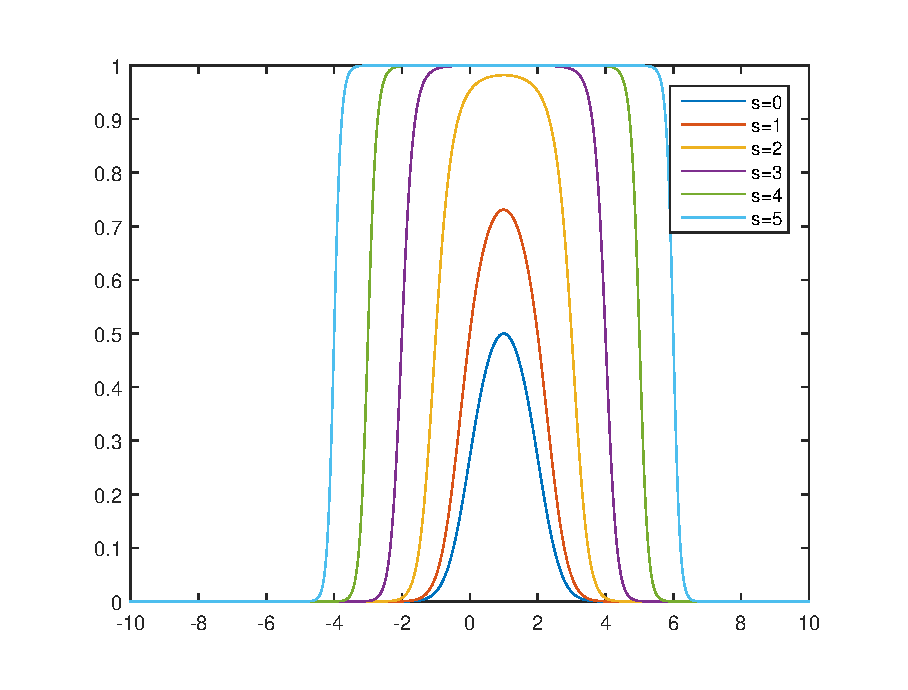
\includegraphics[width=8cm]{./Figures/bell1.eps}
	}
\subfigure[Parametrized by $\alpha$]
	{
	\includegraphics[width=8cm]{./Figures/bell2.eps}
	}
\par\end{centering}
\caption{Penalty term parameterized by $s$ and $\alpha$ }
\end{figure} 
 




 
\end{document}